\documentclass[preprint,5p]{elsarticle}
\usepackage{graphicx}
\usepackage{dcolumn}
\usepackage{bm}  
\usepackage{textcomp}  
\usepackage{amssymb}  
\usepackage{hyperref}
\providecommand{\keywords}[1]{\textbf{\textit{Keywords:}} #1}
\hypersetup{colorlinks=true, urlcolor=blue, citecolor=blue}
\usepackage[displaymath]{lineno}
\linenumbers
\usepackage{dblfloatfix}    % To enable figures at the bottom of page
\begin{document}

\title{\vspace{-15mm}\fontsize{24pt}{10pt}\selectfont\textbf{A Radial Time 
Projection Chamber for $\alpha$ detection in CLAS at JLab}}
\input author_list.tex  

\date{\today}

\begin{abstract}
A new Radial Time Projection Chamber (RTPC) was developed at the Jefferson 
Laboratory to track low-energy nuclear recoils to measure
exclusive nuclear reactions, such as coherent deeply virtual Compton scattering
and coherent meson production off $^4$He. In
2009, we carried out these measurements using the CEBAF Large
Acceptance Spectrometer (CLAS) supplemented by
the RTPC positioned directly around a gaseous $^4$He target, allowing a detection
threshold as low as 12~MeV for $^4$He. This article discusses the design,
principle of operation, calibration methods and performances of this RTPC.
\end{abstract}

\maketitle

\begin{keywords}
Time projection chamber, gas electron multipliers, alpha particles, DVCS, 
Nuclear physics
\end{keywords}

\section{Introduction} \label{sec:level1}

Until recently, the Thomas Jefferson National Accelerator Facility, in 
Newport News, Virginia, USA, has provided high power electron beams of 
up to 6 GeV energy and 100$\%$ duty factor to three experimental Halls (A, B, C) 
simultaneously. The CEBAF Large
Acceptance Spectrometer (CLAS)~\cite{Mecking:2003zu}, located
in Hall-B, was based on a superconducting toroidal magnet and composed of 
several sub-detectors. Figure~\ref{fig:CLAS} shows a three dimensional 
representation of the baseline CLAS spectrometer:
\begin{itemize}
 \item Three regions of Drift Chambers (DC) for the tracking of charged 
       particles~\cite{Mestayer:2000we}.
 \item Superconducting toroidal magnet to bend the trajectories 
       of charged particles, thus allowing momentum measurement with the DC tracking information.
 \item Threshold Cherenkov Counters (CC) for electron identification at momenta 
    $<2.7$ GeV/c~\cite{Adams:2001kk}.
 \item Scintillation Counters (SC) to identify charged hadrons by measuring their 
       time of flight~\cite{Smith:1999ii}.
 \item Electromagnetic Calorimeters (EC) for identification of electrons, 
       photons and neutrons~\cite{Amarian:2001zs}.
\end{itemize}

\begin{figure}[tbp]
\centering 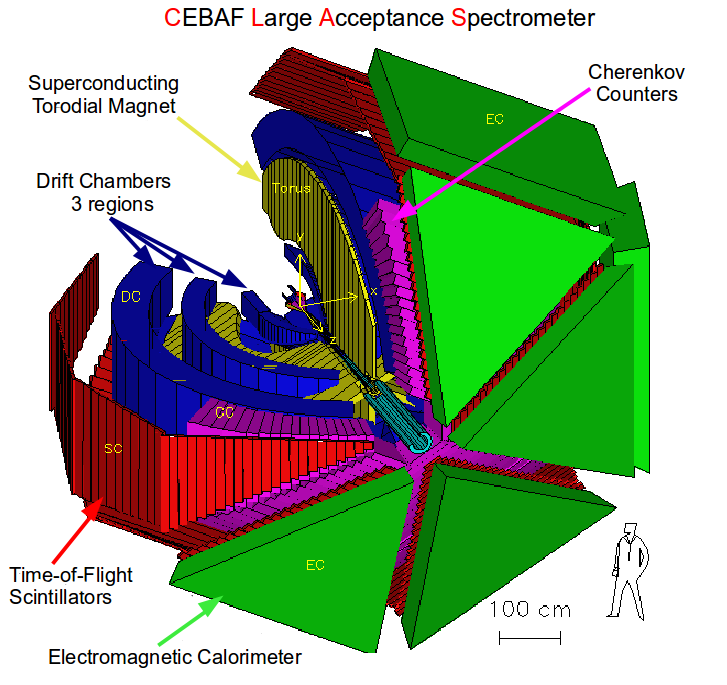
\includegraphics[scale=0.3]{test_clas.png}
\caption{A three dimensional representation of the baseline CLAS setup. The
   full description is given in the text.} \label{fig:CLAS}
\end{figure}

For certain experiments the base CLAS system was complimented with ancillary 
detectors. For example, the measurement of the Deeply Virtual Compton 
Scattering (DVCS) process ($eH \rightarrow e' H' \gamma$, where $H$ is a 
nucleon or nucleus) necessitates an upgrade of the photon detection system.  
Indeed, with a 6 GeV electron beam, the majority of DVCS photons are produced 
at very forward angles, where the acceptance of the EC was poor. To extend the 
detection range, an inner calorimeter (IC) was built for the E01-113 experiment 
in 2005~\cite{Girod:2007aa}. The IC was constructed from 424 lead-tungstate 
(PbWO$_{4}$) crystals, covering polar angles between 5$^{\circ}$ and 
15$^{\circ}$~\cite{Hyon-suk}. To protect the CLAS detector and the IC from the 
large flux of low energy M{\o}ller electrons, a 5~T solenoid magnet was placed 
around the target to shield the detectors.  To detect recoiling $\alpha$ 
particles from the coherent DVCS on Helium, a new radial time projection 
chamber (RTPC) was developed to track low energy nuclear fragments. The 
solenoid field was used to bend tracks and measure momentum of particles in the 
RTPC. The CLAS detector supplemented with both IC and RTPC was used during a 
three months experimental run~\cite{proposal1,proposal2}
in 2009 with a longitudinally polarized electron beam of 130~nA 
and energy of 6.064 GeV incident on a gaseous $^{4}$He target.

The original design of the RTPC was developed for the BoNuS 
experiment at Jefferson Lab which took data with CLAS in 
2005~\cite{Fenker:2008zz}. Significant improvements were made to the RTPC mechanical 
structure and fabrication technique that both increased the acceptance and 
reduced the amount of material in the path of the outgoing particles. 
Moreover, the data aquisition electronic was improved to increase the event 
readout rate. The enhanced design, 
used in the 2009 DVCS experiment, is described in section \ref{sec_design} of 
this paper. The data acquisition system is described in section \ref{sec_readout}, 
the calibration methods in section \ref{sec_calib} and the tracking algorithm in section
\ref{sec_tracking}. Finally, the overall performances
of the RTPC are described in section \ref{sec_perfor}.

\section{RTPC design} \label{sec_design}

With a 6 GeV incident electron energy, the recoiling $^{4}$He nuclei from 
coherent DVCS have an average momentum around 300~MeV/c (12~MeV kinetic 
energy). Such low energy $\alpha$ particles are stopped very rapidly, so the 
RTPC was designed to be as close as possible to the target and fit inside the 
230~mm diameter shell and cryostat wall of the solenoid magnet bore of the 
CLAS.

\begin{figure}[tb]
\centering
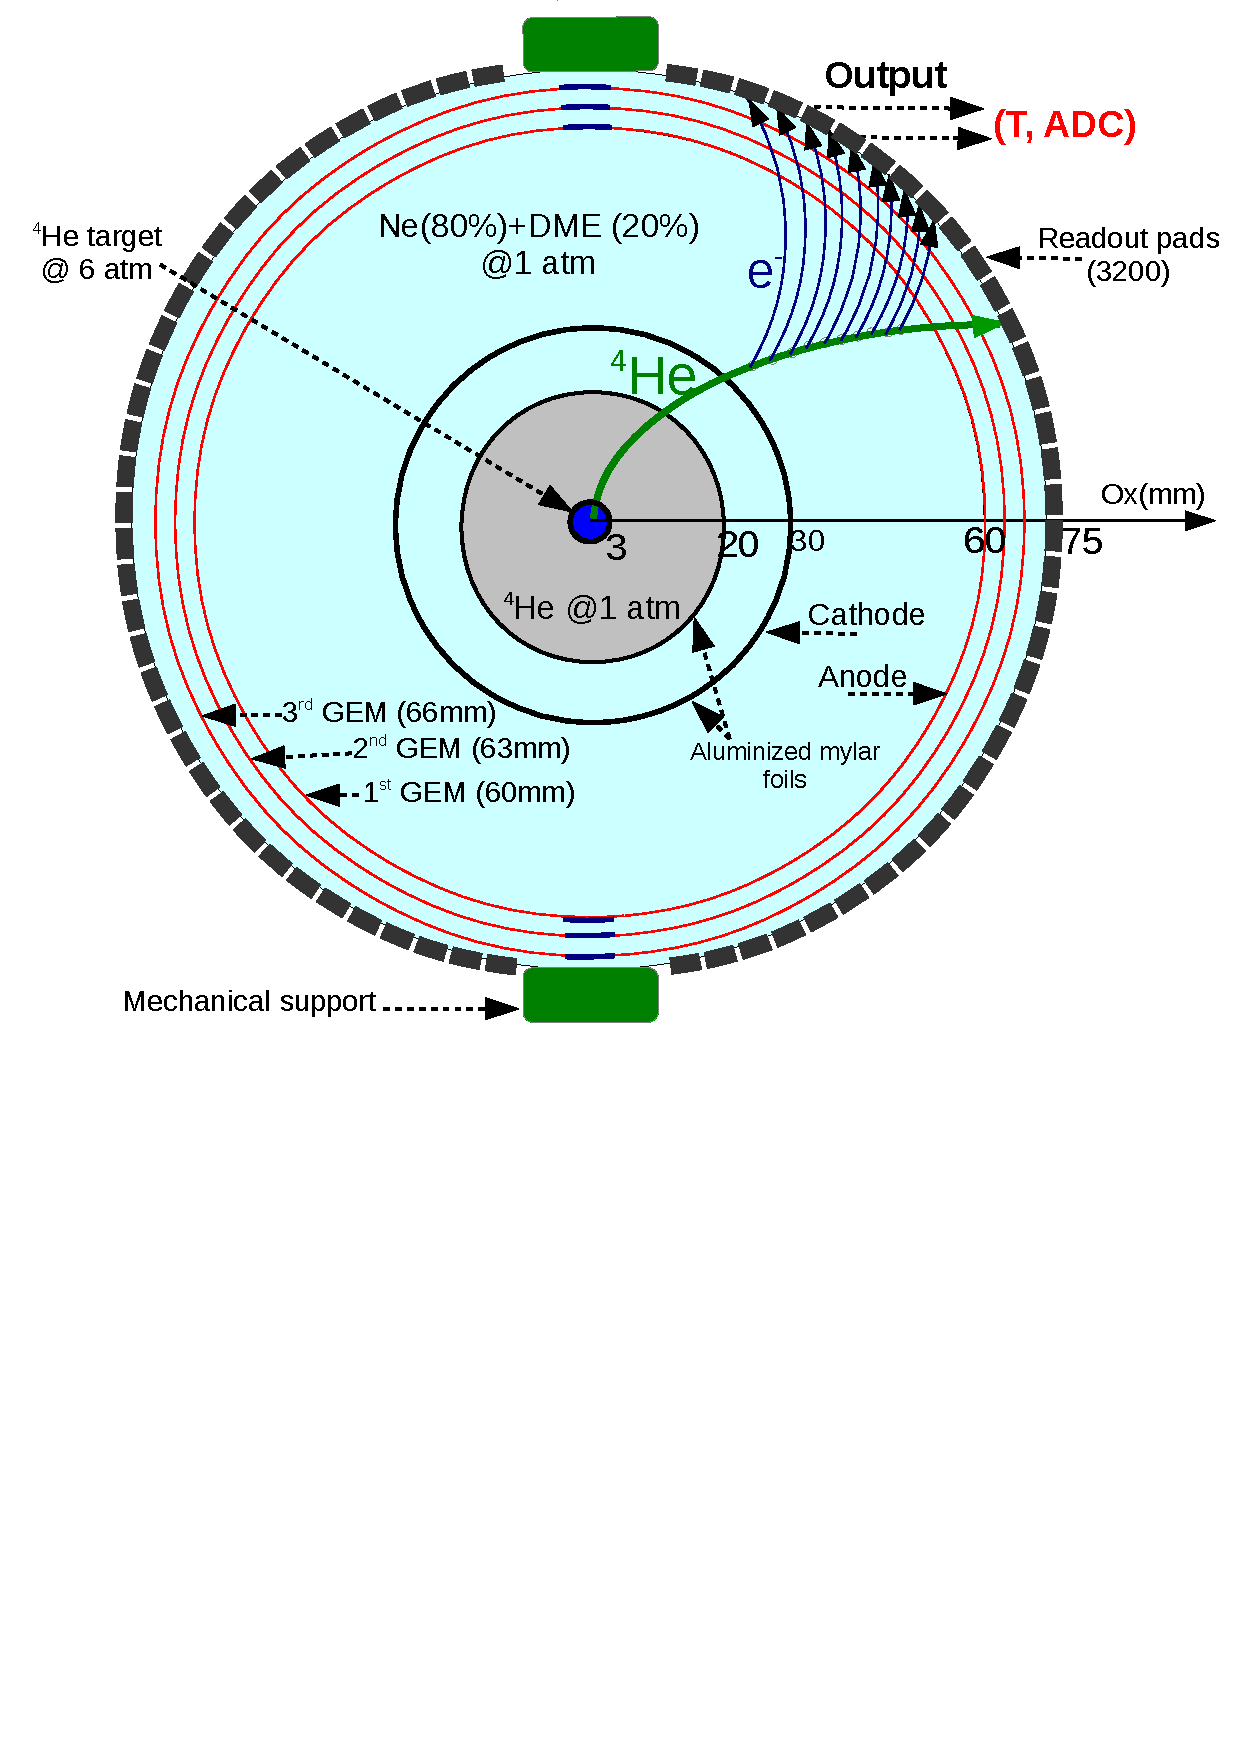
\includegraphics[{trim={0 12cm 0 0},clip, scale=0.4}]{RTPC_1_all.pdf}
\caption{Schematic drawing of the CLAS RTPC in a plane perpendicular to the beam 
direction. See text for description of the elements.} \label{fig:RTPC_1_4}
\end{figure} 

The new CLAS RTPC is a 250~mm long cylinder of 158~mm diameter, leaving just enough 
room to fit pre-amplifiers between the RTPC outer shell and the solenoid. The 
electric field is directed perpendicularly to the beam direction, 
such that drifting electrons are pushed away from the beam line. These electrons 
are amplified by three layers of semi-cylindrical gas electron multipliers 
(GEM)~\cite{Sauli:2016eeu} and detected by the readout system on the external 
shell of the detector as illustrated in Figure~\ref{fig:RTPC_1_4}. The RTPC is 
segmented into two halves with independent GEM amplification systems that cover 
about 80\% of the azimuthal angle.

We detail here the different regions shown in Figure~\ref{fig:RTPC_1_4} 
starting from the beam line towards larger radius:\\
\begin{itemize}
  \item The 6~atm $^4$He target extends along the beamline forming the detector 
     central axis. It is a 6~mm diameter Kapton straw with a 27~\textmu{}m wall 
     of 292~mm length such that its entrance and exit 15~\textmu{}m aluminum windows 
     are placed outside of the detector volume. The detector and the target are 
     placed in the center of the solenoid, 64~cm upstream of the CLAS center.
   \item The first gas gap covers the radial range from 3~mm to 20~mm. It is 
      filled with $^{4}$He gas at 1~atm to minimize secondary interactions from
      M\o{}ller electrons scattered by the beam. This region is surrounded by 
      a 4 \textmu{}m thick window made of grounded aluminized Mylar.
   \item The second gas gap region extends between 20~mm and 30~mm and is 
      filled with the gas mixture of 80$\%$ neon (Ne) and 20$\%$ dimethyl ether 
      (DME).  This region is surrounded by a 4~\textmu{}m thick window made of 
      aluminized Mylar set at $-4260$~V to serve as the cathode.
   \item The drift region is filled with the same Ne-DME gas mixture and 
      extends from the cathode to the first GEM, 60~mm away from the beam axis.  
      The average electric field in this region is perpendicular to the beam 
      and about 550~V/cm.
   \item The electron amplification system is composed of three GEMs located at 
      radii of 60, 63 and 66~mm. In this configuration, the first GEM layer 
      serves as the anode and each subsequent GEM is set at a lower voltage to
      obtain a strong ($\sim$1600~V/cm) electric field between the GEM foils. A 
      275~V bias is applied across each GEM for amplification.
   \item The readout board has an internal radius of 69~mm and collects charges 
      after they have been multiplied by the GEMs. Pre-amplifiers are plugged 
      directly on its outer side and transmit the signal to the data 
      acquisition electronics.
\end{itemize}

\begin{figure}[tbp]
\centering
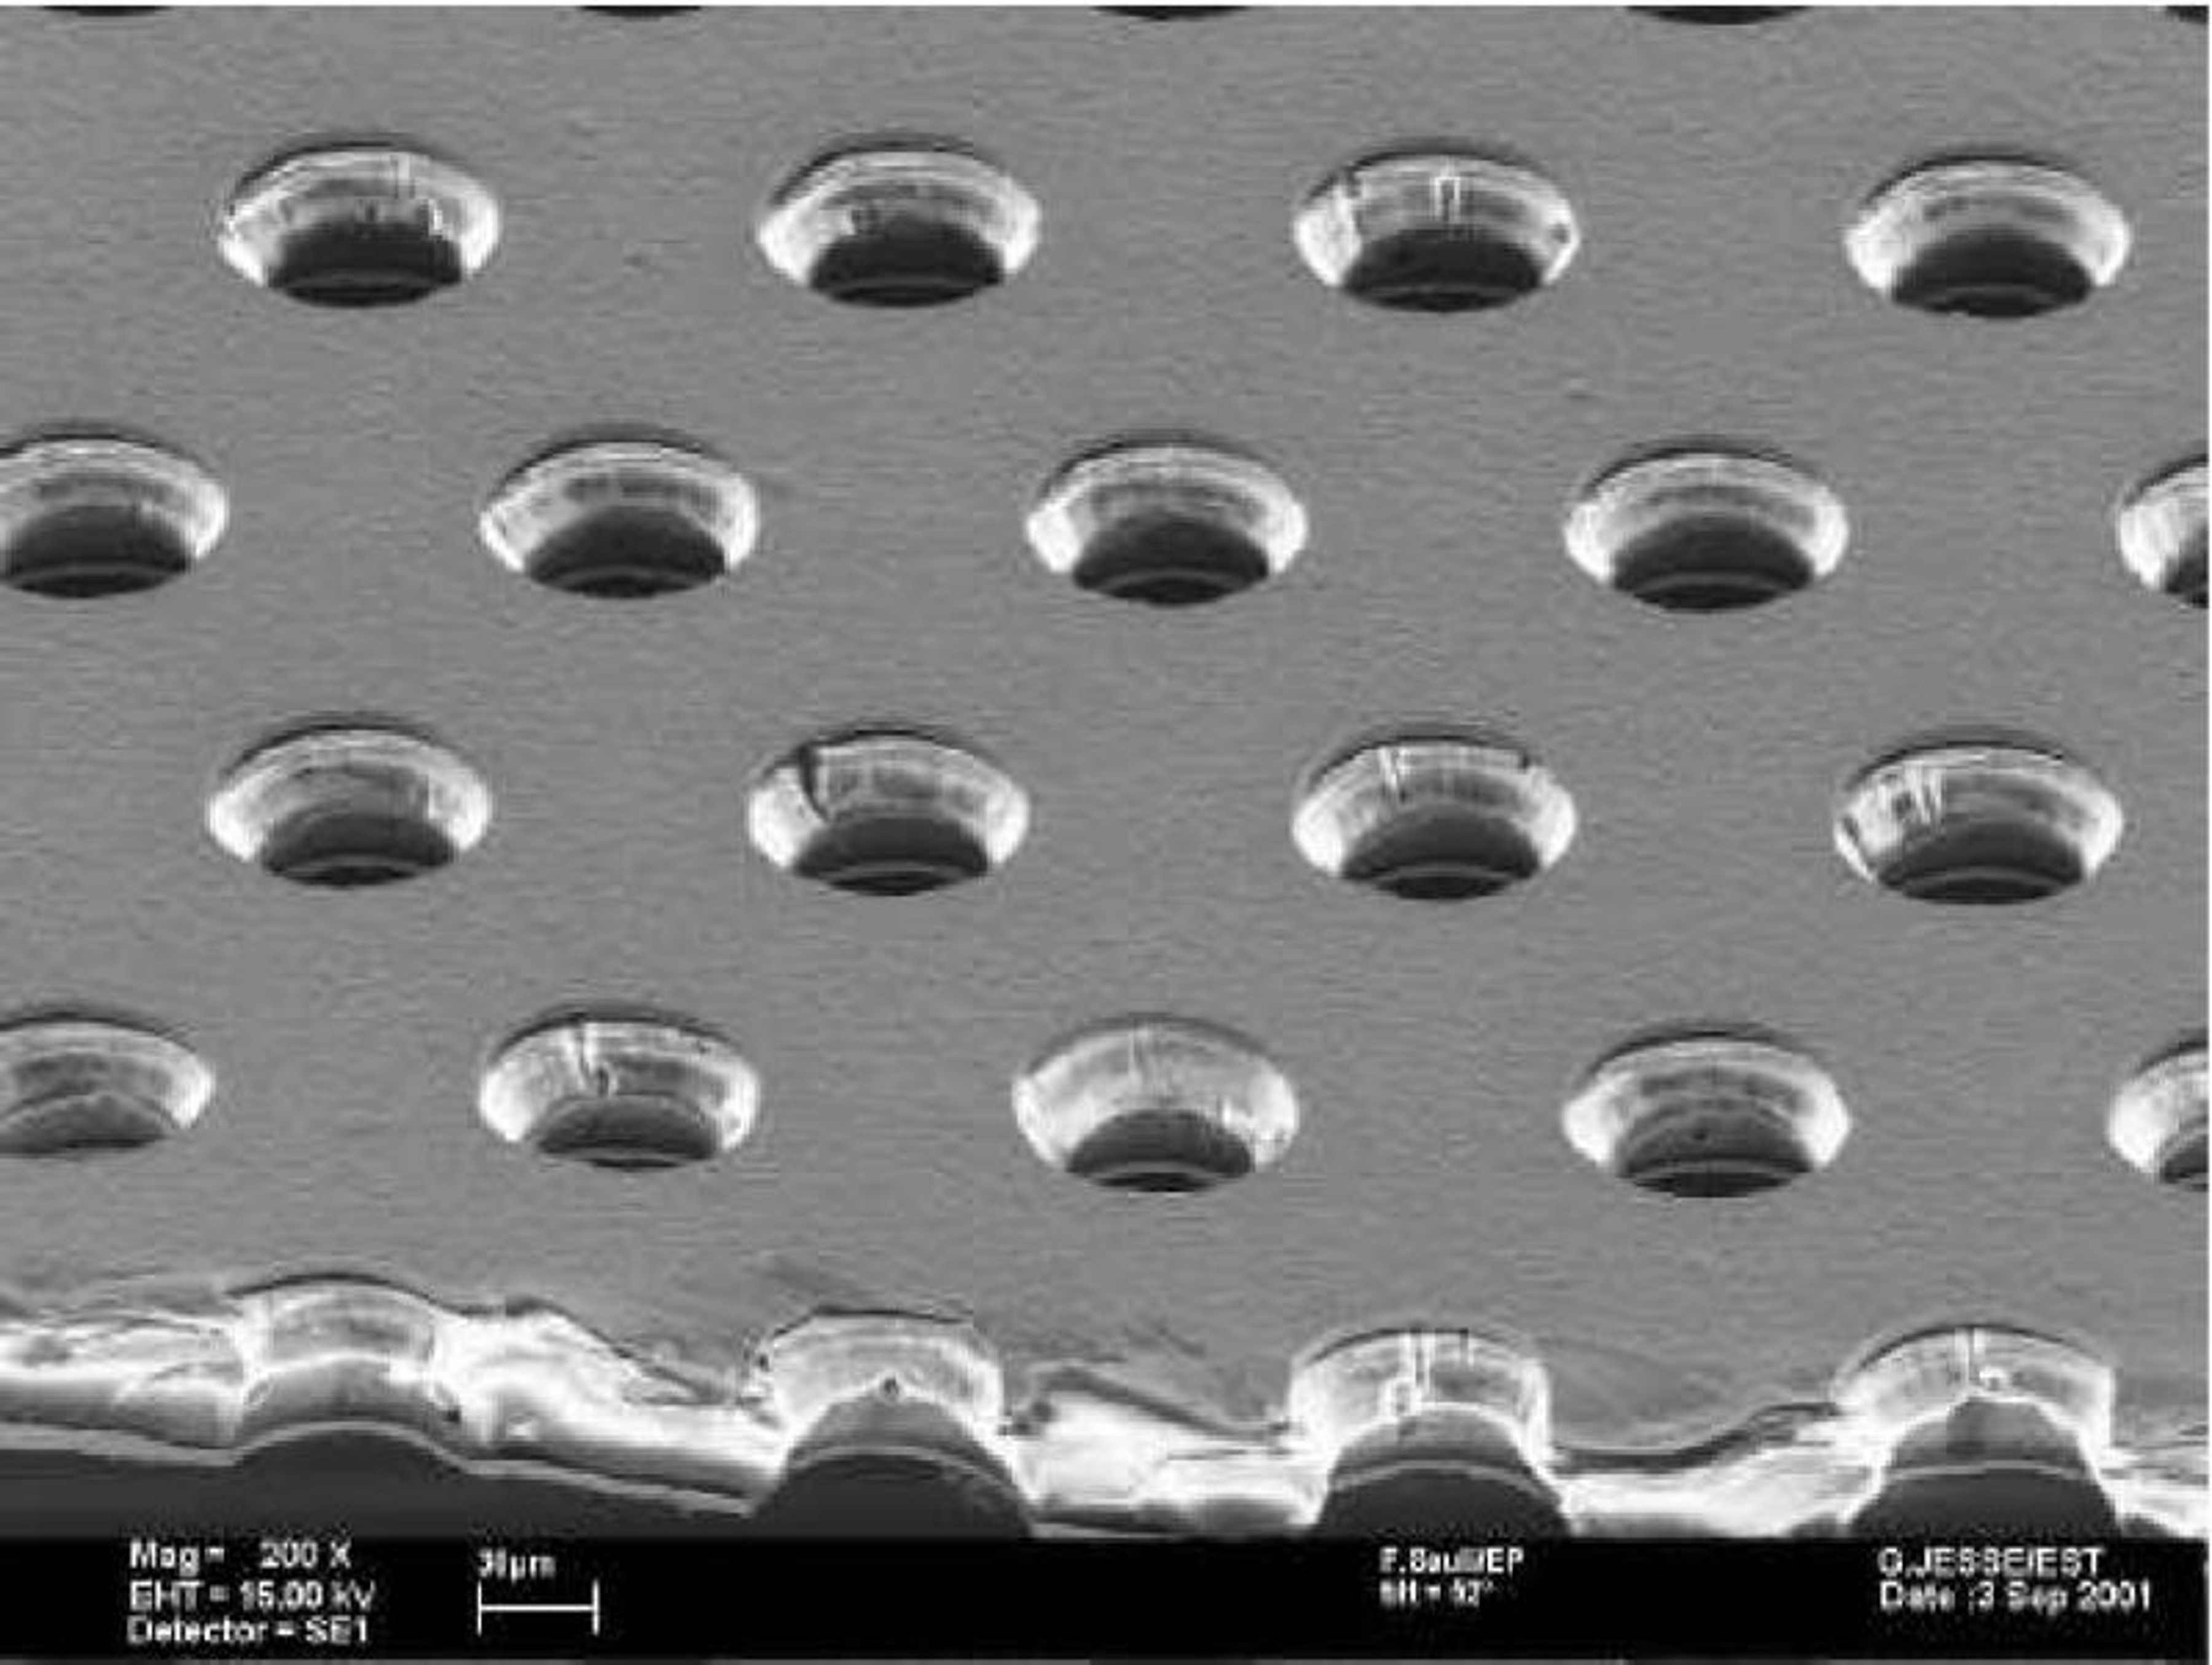
\includegraphics[scale=0.70]{GEM_photo.jpg}
\caption{Image of a typical GEM foil similar to the one used for our RTPC 
\cite{Sauli:2016eeu}.} 
   \label{fig:GEMs}
\end{figure}

The GEM technology has been chosen for the flexibility of the GEM foils,
which can be easily used to produce a curved amplification surface. Also, GEMs 
are known to have relatively low spark rate~\cite{Bachmann:2000kj}, which is 
important when trying to detect highly ionizing slow nuclei that deposit large 
amount of energy. The GEMs for this RTPC are made from a Kapton insulator 
layer, 50~\textmu{}m thick, sandwiched between two 5~\textmu{}m copper 
layers\footnote{The GEM foils were produced by Tech-Etch, Inc.}. The mesh of 
each GEM layer is chemically etched with 50~\textmu{}m diameter holes with 
double-conical shapes as illustrated in Figure~\ref{fig:GEMs}. The potential 
difference applied between the two copper layers of the GEM creates a very 
strong electric field in each hole leading to high ionization and 
amplification. 

The drift gas used in the experiment is a 80-20\% Ne-DME mixture. This choice 
has been made in order to balance the energy deposit, which is critical
for proper particle identification, with a reasonable
Lorentz angle. Calculations using the MAGBOLTZ program~\cite{Biagi:1999nwa} 
showed that with the 5~T solenoidal magnetic field, we would have a Lorentz 
angle of about 23$^\circ$ with this gas mixture.

The main structural improvement compared to the 2005 RTPC~\cite{Fenker:2008zz} 
was to obtain a better support structure for the GEM foils. In the previous version,
the RTPC was essencially composed of two independent half-cylinder separated
by their own structures. In this design, the installation of the GEMs was not very practical
and wrinkles were visibles on the GEM surfaces. To allow for a better installation 
and, at the same time, keep the mechanical structure out of the drift volume, 
the present design is based on self supporting GEM cylinder. We 
realized these cylinders by using fiber glass rings glued to 
each ends of the GEM foils in order to 
instal them independently in the RTPC after gluing and soldering operations. The 
rigidity of the GEM foils was enough for the structure to be self-supporting 
and only the upstream end of the cylinder was fixed to the main mechanical 
support structure. This design only left a light fiberglass ring in the 
downstream end, reducing to a minimum secondary interactions.

\section{Readout System} \label{sec_readout}

\begin{figure}[tb]
   \centering
   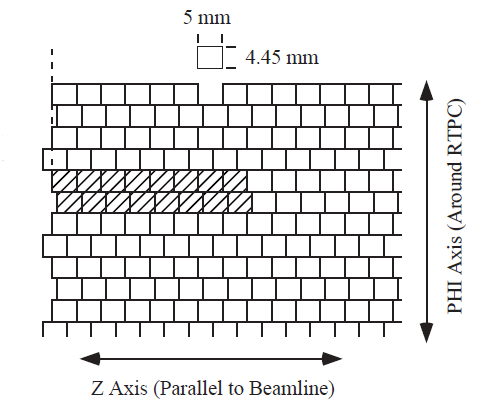
\includegraphics[scale=0.55]{PADs.png}
   \caption[]{A schematic representation of the readout pads. The 
   shaded sixteen pads are a group of pads that are connected to the same 
pre-amplifier.} \label{fig:PADs}
\end{figure}

The RTPC electron collection system had 3200 readout pads. These elements were
located at the end of the amplification region, 69~mm from the central axis.
Figure \ref{fig:PADs} illustrates the configuration of the 5 by 4.45~mm pads,
where the shift between the rows was implemented to reduce aliasing. Each half 
of the RTPC had 40 rows and 40 columns of pads. The shaded region in 
Figure~\ref{fig:PADs} shows how pads were grouped to 16 channels pre-amplifier 
boards. The pre-amplifier boards, already employed in the BoNuS 
RTPC~\cite{Fenker:2008zz}, serve the dual purpose of inverting the RTPC signals 
polarity -- from negative to positive -- to match the requirements of the 
subsequent readout system, and driving the 6~m long ribbon cable that connects 
to it.

The readout system was an upgraded version of the original BoNuS RTPC system~\cite{Fenker:2008zz}, 
based ALICE-TPC front end electronic boards (FECs)~\cite{ALICE-FEE}. 
Each FEC hosted 128 channels, providing amplification and digitization of the 
input signals. For each event, 100 samples/channel were digitized by the ALTRO 
ASIC~\cite{EsteveBosch:2003bj}, operated at 10 MHz sampling frequency. In order 
to reduce the data size, the system was operated in zero-suppression mode, 
keeping data from $N_{PRE}=3$ samples before threshold crossing on the rising 
edge to $N_{POST}=3$ samples after threshold crossing on the falling edge. 
The threshold level was set on each channel just above the noise level.

A new custom backplane was developed to connect FECs to the Readout Control 
Unit (RCU)~\cite{RCU}, allowing fast (200 MB/s) communication between the 
boards. The RCU board, used to distribute the trigger signal to different FECs 
and read data, was equipped with a fast optical link for data transferring to 
the main event builder. These features, together with the ``block-transfer'' 
readout mode making use of the FECs multi-event buffer, allowed to reach a 
signifantly higher readout-rate compared to the original BoNuS system. During 
the 2009 run, the system was successfully 
operated with a DAQ rate of 3.1 kHz and a live time of 70~\%, for a 
luminosity of about $10^{34}$~cm$^{-2}\cdot$s$^{-1}$ and a beam energy of 
6.064~GeV, to be compared with the 500 Hz obtained with the first BoNuS detector at similar run conditions.

During data reconstruction, the acquired samples were processed to obtain, 
for each readout pad, the accumulated charge (ADC) and the pulse time (T). Since 
pulse time was obtained as the time-stamp of the first sample above threshold, 
referred to the trigger time, the resolution was equivalent to the ALTRO 
sampling time of 100~ns.

\section{Calibration} \label{sec_calib}

The timing information collected for each signal above threshold
was used to infer the origin of the ionization electrons and 
then the trajectory of the detected particle. The recorded ADCs were used to reconstruct 
the deposited energy per unit of length ($\small{\frac{dE}{dX}}$) which, 
together with the momentum calculated from the trajectory, enabled the particle 
identification. 

In this section we will detail the methods used to calibrate the drift time,
drift paths and gains of the detector. Drift time and paths were initially
calculated using the MAGBOLTZ~\cite{Biagi:1999nwa} program, then refined using
data to account for variations of the run conditions. We assume 
cylindrical symmetry in the chamber for the calibration of the drift parameters, 
such that do not depend on the azimuthal angle $\phi$. The initial MAGBOLTZ
calibration was improved through several iterations of the
data driven process described below, with each time an increasing number of tracks 
reconstructed in the RTPC. The figures presented in this section
are the ones obtained while performing the last iteration of this
calibration process.

\subsection{Maximum Drift Time Parametrization}

%To be rewritten!!!
After the ionization, the released electrons drift to the cylindrical detection 
plane under the effect of the electric field. The electrons released close to 
the cathode take the most time to reach the readout pads, the cylindrical 
symmetry indicates that this maximum drift distance is the same for all tracks.  
We illustrate this in Figure~\ref{fig:RTPC_signals}, where we depict a typical 
$^{4}$He track. Due to the non-perfect experimental conditions, in particular 
possible contamination of our gas mixture, the drift speed changed during the 
three months long experimental run\footnote{We had to increase the gas flow 
during the experiment due to a small leak in the RTPC, which concurred to 
the large shift of drift time observed around run number 61600. While our 
gas system was kept slightly over atmospheric pressure to limit 
contamination from air or other external gases, it is likely that this leak was 
the source of modification of the drift speed.}. This can be calibrated by 
finding drift speed as function of experimental run-number. By measuring a 
reference time, we can therefore infer the drift speed of the electrons in the 
RTPC, by: $\textnormal{drift time} = \frac{\textnormal{drift path 
length}}{\textnormal{drift speed}}$.

\begin{figure}[tb]
\centering
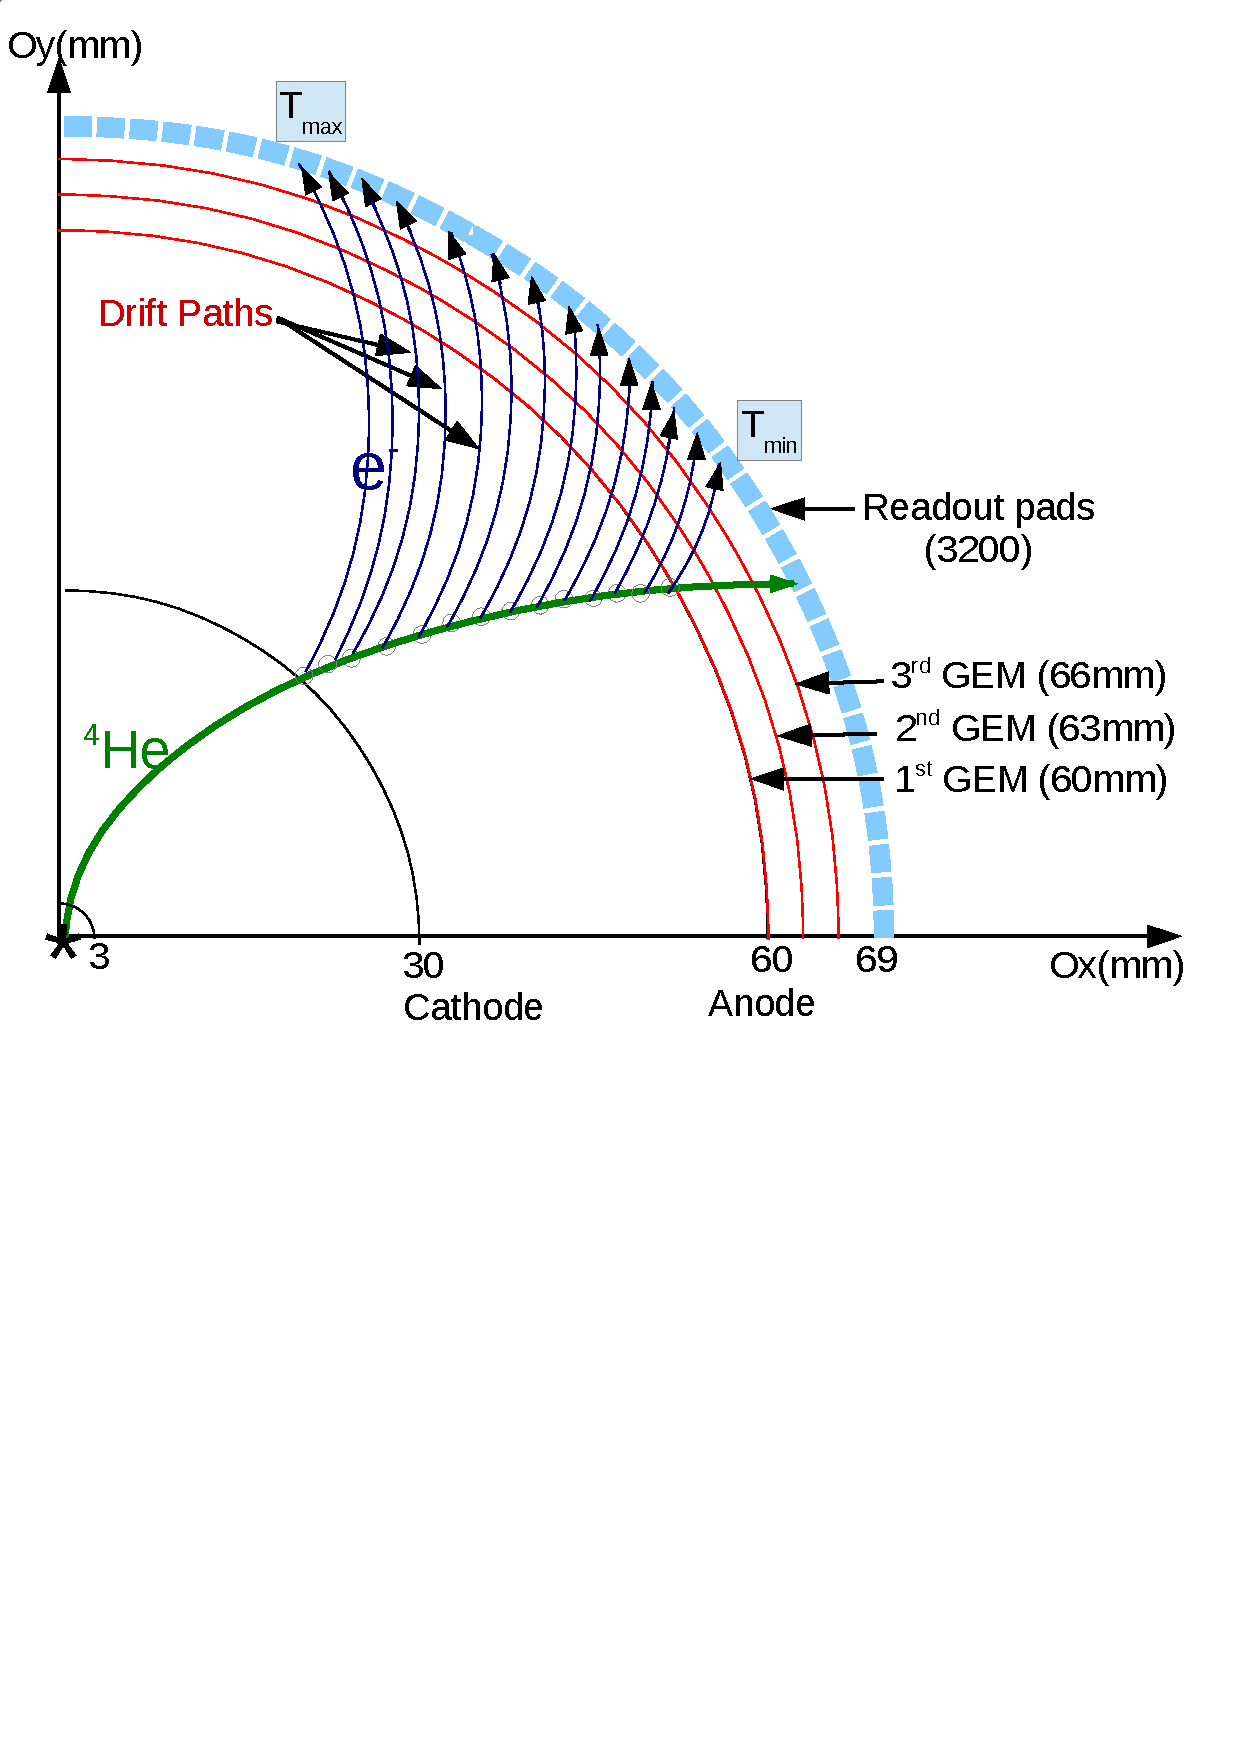
\includegraphics[{trim={0 12cm 0 0},clip, scale=0.4}]{RTPC_1_4.pdf}
\caption[]{A schematic drawing of a $^{4}$He track (in green) traversing the 
drift region, with the drift paths followed by the electrons (in black). } 
\label{fig:RTPC_signals}
\end{figure}

Figure~\ref{fig:TDC_profile} presents the time profile of hits from identified 
tracks in one z-bin along the detector in one experimental run. We can clearly 
observe the dropping edge expected from geometrical considerations. In order to 
avoid the statistical fluctuations on finding the maximum drift time 
($T_{max}$) from the time profile, we define a more stable value, i.e., 
$T_{max/2}$, at which the dropping edge passes half the maximum number of hits 
in the histogram. This value was measured in bins along the 200~mm RTPC's 
length to take into account variations in the electric and magnetic field in 
the RTPC (see Figure~\ref{fig:RunNumber_61551_TDCmax_Zslice}). 

\begin{figure}[tb]
\centering
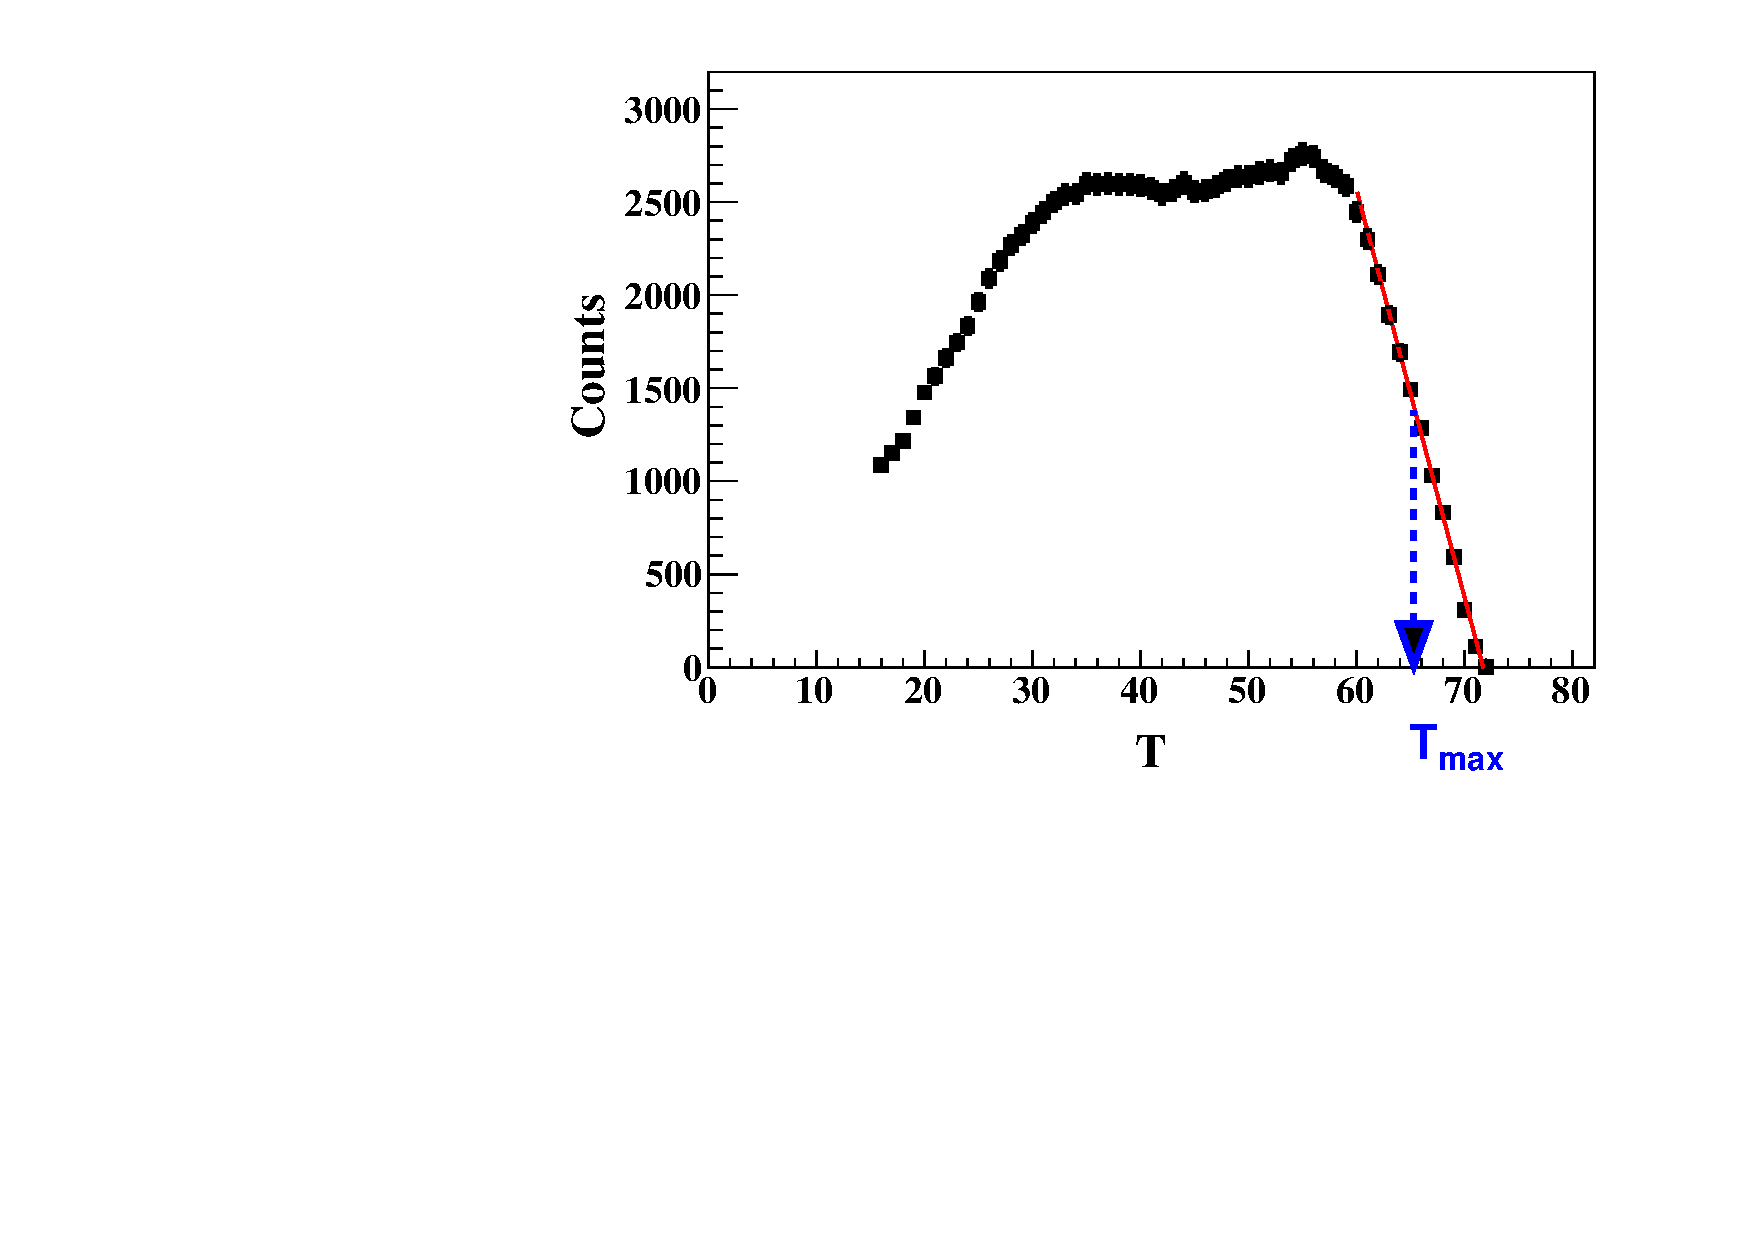
\includegraphics[scale=0.42]{hits_time_profile.pdf}
\caption[]{Time distribution of the hits in one z-bin along the RTPC in one 
experimental run. Trigger time is defined as T=15, the time unit is the ALTRO 
sampling time of 100~ns.} \label{fig:TDC_profile}
\end{figure}

\begin{figure}[tb]
\centering
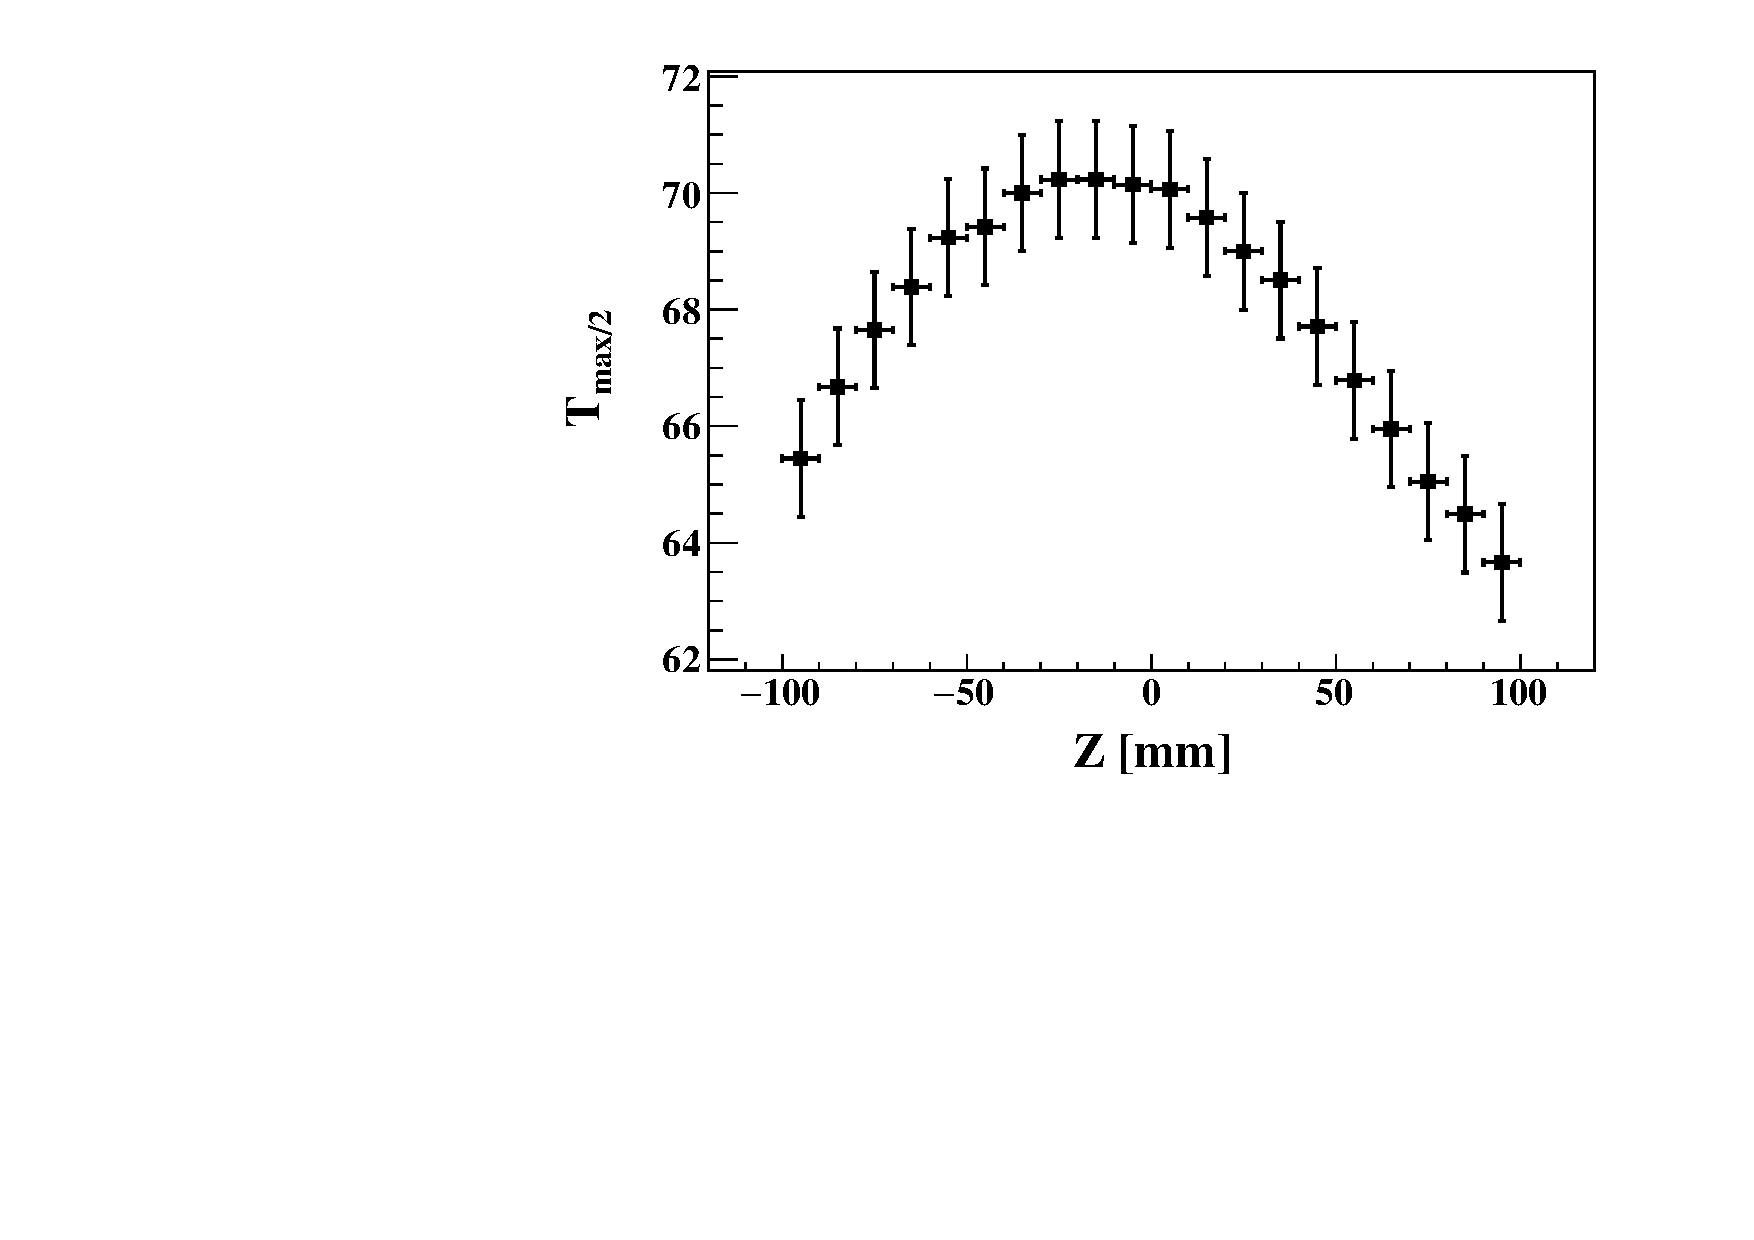
\includegraphics[scale=0.42]{RunNumber_61452_TDCmax_Zslice.pdf}
\caption{Maximum time of collected hits as a function of the track
              position on the $z$-axis for one experimental run. } 
\label{fig:RunNumber_61551_TDCmax_Zslice}
\end{figure}

Figure~\ref{fig:Drift_run_number_1} shows the $T_{max/2}$ values for individual 
runs (approximately 2 hours long). We observe significant change in the drift 
speed before and after run 61600, while variations within these periods are 
around 2\%. 

\begin{figure*}[tb]
\centering
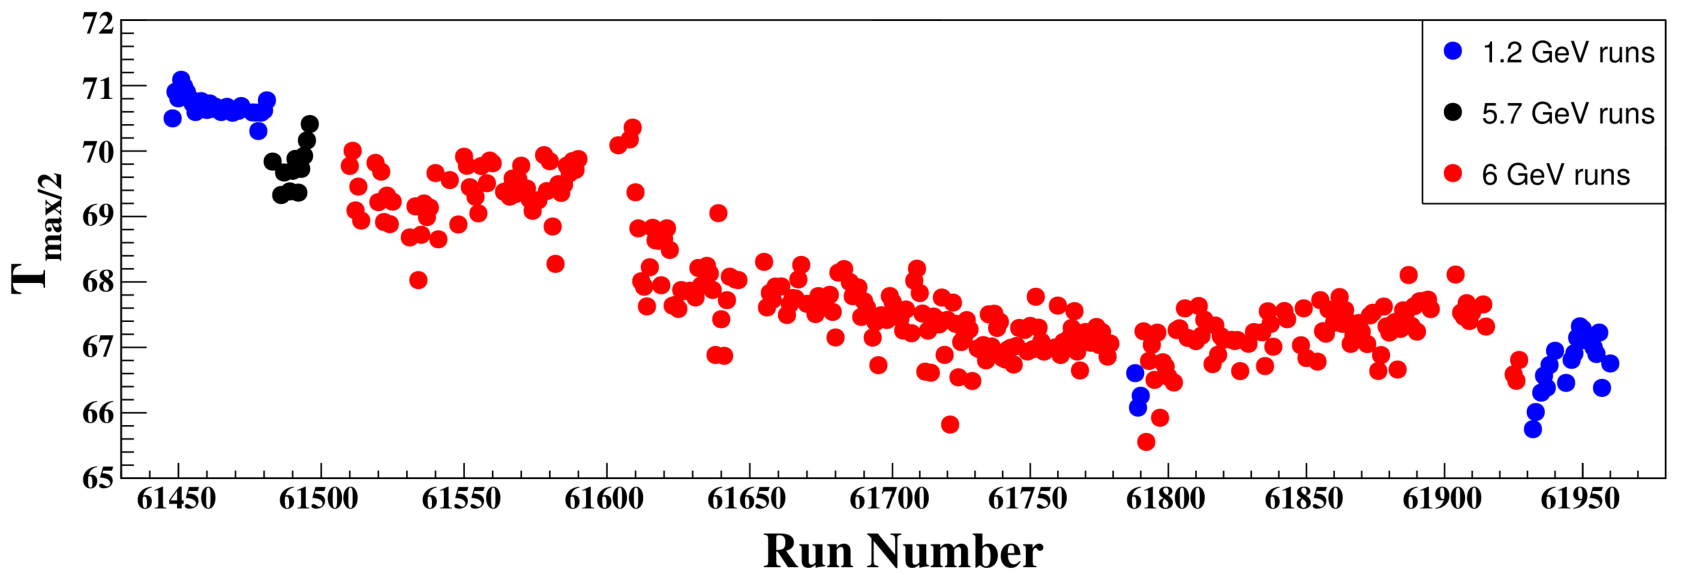
\includegraphics[width=17.5cm]{Drift_run_number.pdf}
\caption{$T_{max}$ versus the experimental run numbers.} 
\label{fig:Drift_run_number_1}
\end{figure*}

In summary, we obtain from our calibration a parametrization of the drift speed 
as a function of both position along the beam axis and the run number.  These 
functions were extracted for our entire data set and implemented in the track 
reconstruction code.
   
\subsection{Drift Path Calibration}

The drift path is the trajectory followed by the electrons released through 
ionization in the gas. We calculated them with
MAGBOLTZ~\cite{Biagi:1999nwa}, but it requires knowledge of the detector's 
geometry, gas mixture composition, and of course the electric and magnetic 
fields over the whole volume of the detector. We used this calculation as a 
first calibration, but, as can be seen with the drift speed, conditions in the 
chamber were changing over time. Moreover, the 4 \textmu{}m foil used as a cathode 
is easily deformed, such that we expect the geometrical accuracy to be of few 
millimeters, directly impacting our knowledge of the electric field. These 
problems, already encountered for the BoNuS RTPC 
calibration~\cite{Fenker:2008zz}, motivated the acquisition of specific 
calibration runs. These were taken with a lower energy electron beam (1.204 and 
1.269 GeV) to enhance the cross section of the elastic scattering 
($e^{4}$He$\rightarrow e^{4}$He). In this process, the measurement of
the electron kinematics allows to calculate directly the kinematics of the Helium nucleus. 
By comparing the calculated momentum and angle of the recoil alpha particle to the 
measurement in the RTPC, we tuned the drift paths independently of our 
knowledge of the chamber's conditions.

Based on the kinematics of the electrons in the calibration data, we generated 
the Helium nucleus in our RTPC GEANT4 simulation~\cite{GEANT4}. Then,
we compared the calculated GEANT4 trajectory of the Helium nuclei to 
the hits measured in the chamber. To perform this drift path extraction, 
we made a first approximation assuming a linear dependence between the radius 
of emission of the charge and its time of detection, and then refined our 
result. Because of the magnetic field, the drift paths in RTPC are not linear 
but the curvature is small and the refining  process converged already on the 
second iteration.

At the end of the extraction procedure, the azimuthal difference between the 
detection pad and the ionization point ($\Delta\phi$) was extracted as a 
function of time. In Figure~\ref{fig:DELTA_PHI_TDC}, we show the resulting data 
points for one bin in z-coordinate of the RTPC, where the drift path is easily 
identified and eventually fitted for implementation in our reconstruction code.

\begin{figure}[tb]
\centering
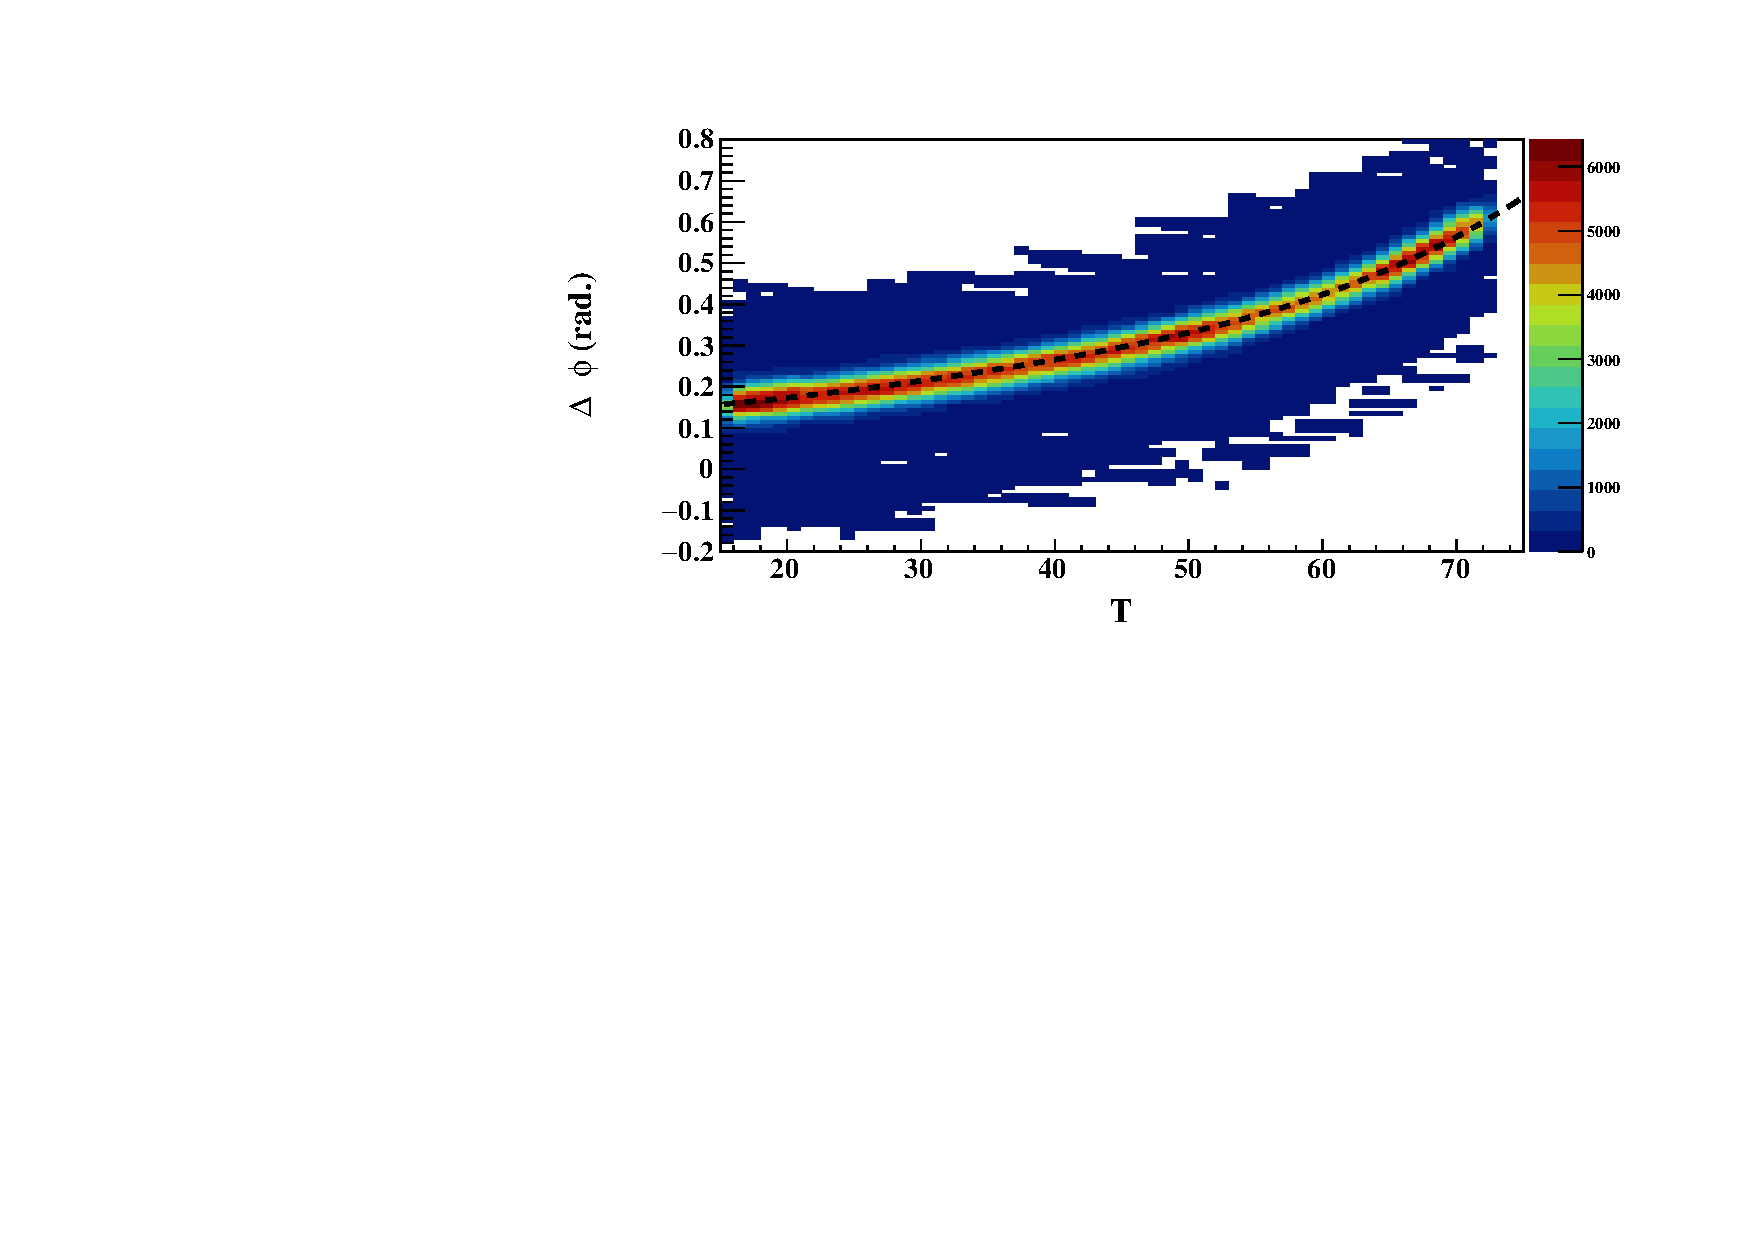
\includegraphics[scale=0.46]{FitResult_p2_11.pdf}
\caption{$\Delta \phi$ versus T distribution for tracks
from one bin in longitudinal position along the RTPC. The black line represents 
the final drift paths in this bin.}
\label{fig:DELTA_PHI_TDC}
\end{figure}

To verify the stability of the drift paths, this procedure was carried out 
using both the 1.204 GeV data from the beginning of the run period and the 
1.269 GeV data from the end of the run period (shown in blue on 
Figure~\ref{fig:Drift_run_number_1}). We found very similar drift paths for the 
two data sets and concluded that any changes in the system only significantly 
affected the drift speed.

\subsection{Gain Calibration}

To calibrate the gains, we compared the experimental ADCs to the energy 
deposited for each pad individually in GEANT4 by similar simulated tracks 
(using the same elastic events as for the drift paths calibration). This 
requires a detailed simulation, including the drift paths and the diffusion of 
the charges along the path before reaching the pad to 
match the experimental data. We implemented in the GEANT4 simulation the
drift path we obtained from the calibration described above and implemented an ad 
hoc diffusion to match the average number of hits recorded in the simulation with
the one from experimental data. To perform this step properly, we implemented in
the simulation the details of the DAQ process to record hits. 

We then compared this simulation to experiment on an event by event basis as 
shown in Figure~\ref{fig:EVENT_adc_tdc}. The gain for each pad was calculated 
as the ratio of the measured ADCs to the simulated deposited energy. This 
provided our initial set of gains for each pads and it was applied to the 
experimental data. However, after this calibration some pads recorded lower ADCs 
than expected. So, we added a correction factor obtained by comparing  
the energy deposit on a given pad to its neighbours. To do so, we compared, for 
each track, the energy deposit on a pad to the energy deposit in the whole track. 
The gain correction factors are extracted by averaging this ratio for a sample 
of elastic events. Final results are shown in Figure~\ref{fig:dedx_p_exp_2nd}, where energy 
loss of particles is plotted against momentum over charge ratio. One can 
clearly see the band for $^4$He in its expected position\footnote{The lower peak 
   in the left module of the RTPC comes from an unidentified problem in this half 
   of the detector that concerns 7\% of all the elastic events. 
   Our best guess is that these events are linked with a high voltage supply 
   issue, that would sometimes bring the GEM gain down. These events pass all 
   the elastic requirements and we found nothing that differenciates them 
   from other events but their low recorded ADCs. For 
   the calibration procedures, these events were therefore excluded.}.

\begin{figure}[!t]
   \centering
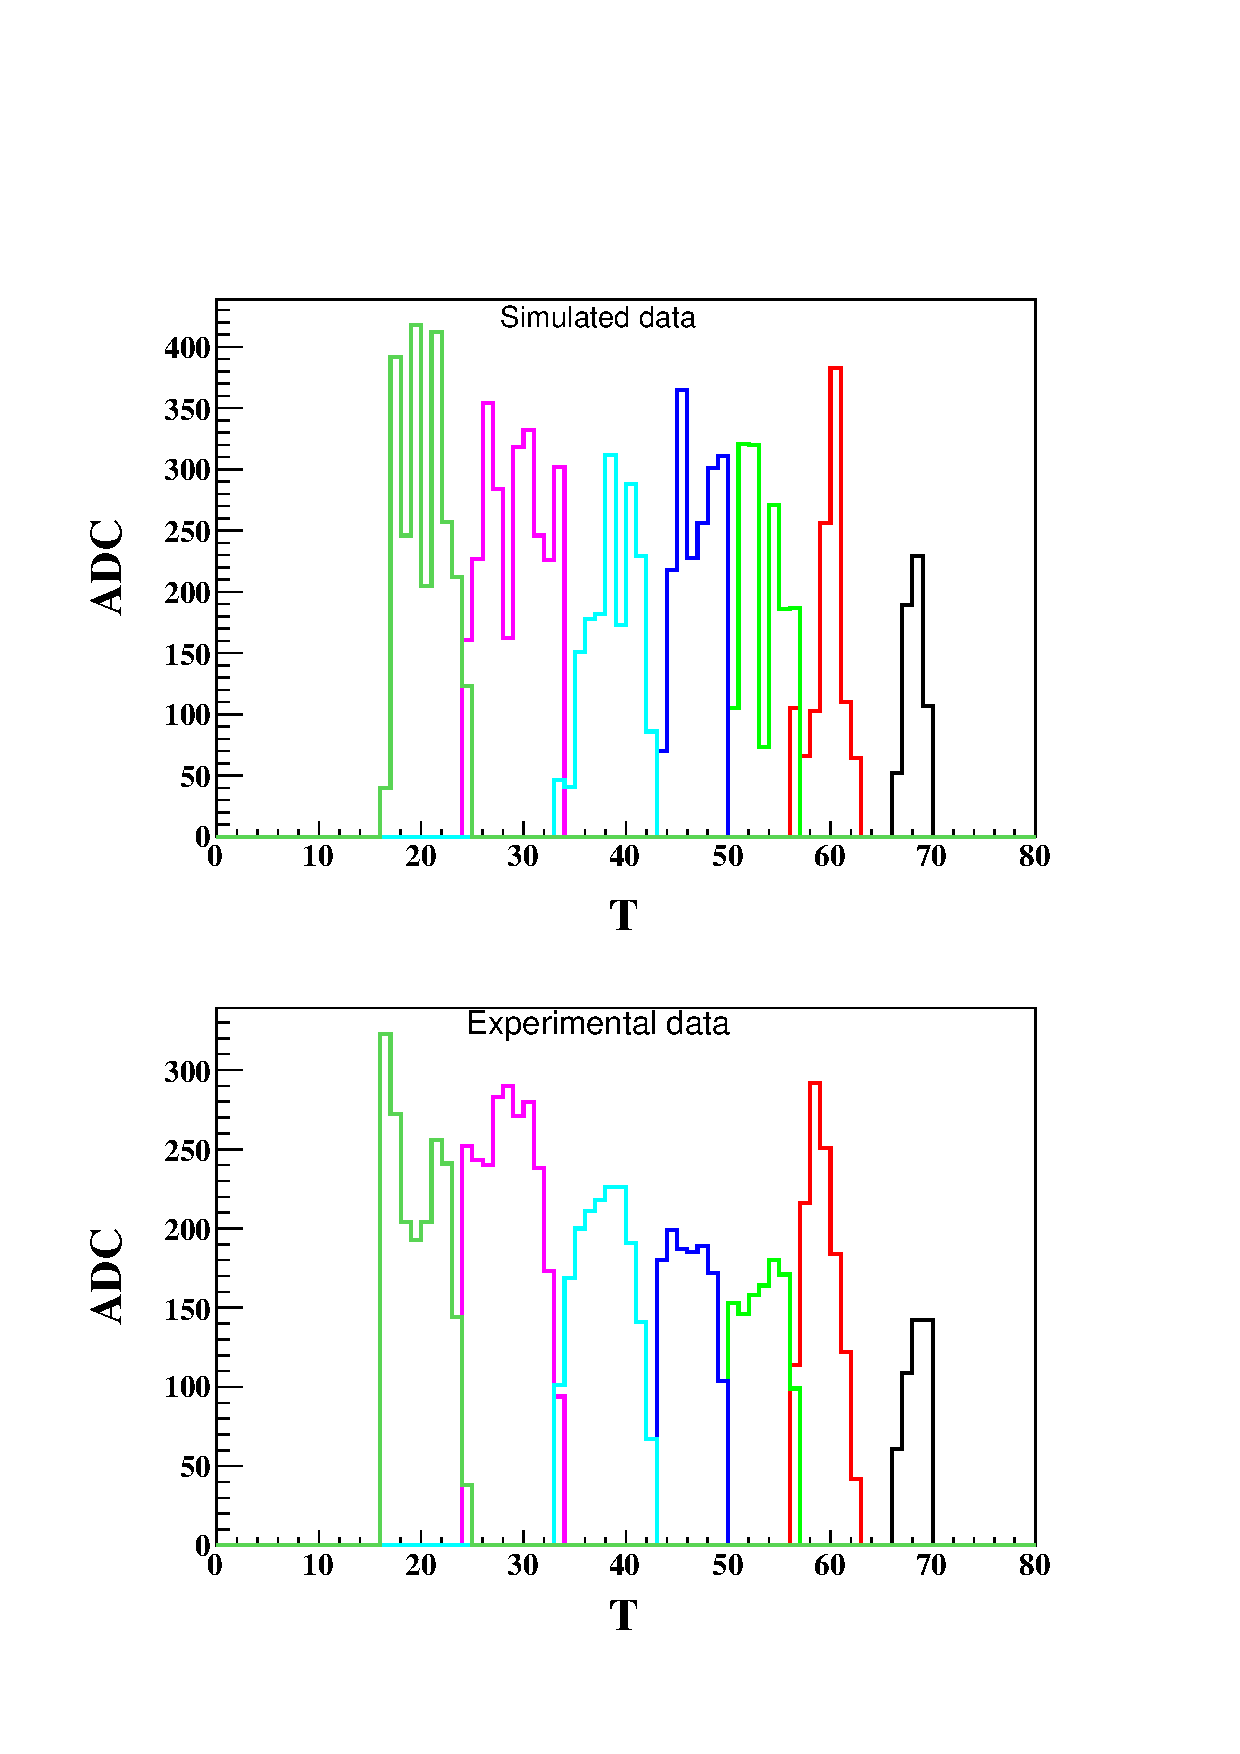
\includegraphics[scale=0.42]{Event_ADC_Graph_8799283.pdf}
\caption{Simulated (upper) and experimental (lower) ADC and T distributions 
of a single track. The different colors indicate the signals from different pads, 
the same color in the top and bottom figure indicate that the signal was registered
on the same pad.}
\label{fig:EVENT_adc_tdc}
\end{figure}

\begin{figure*}[!h]
\centering
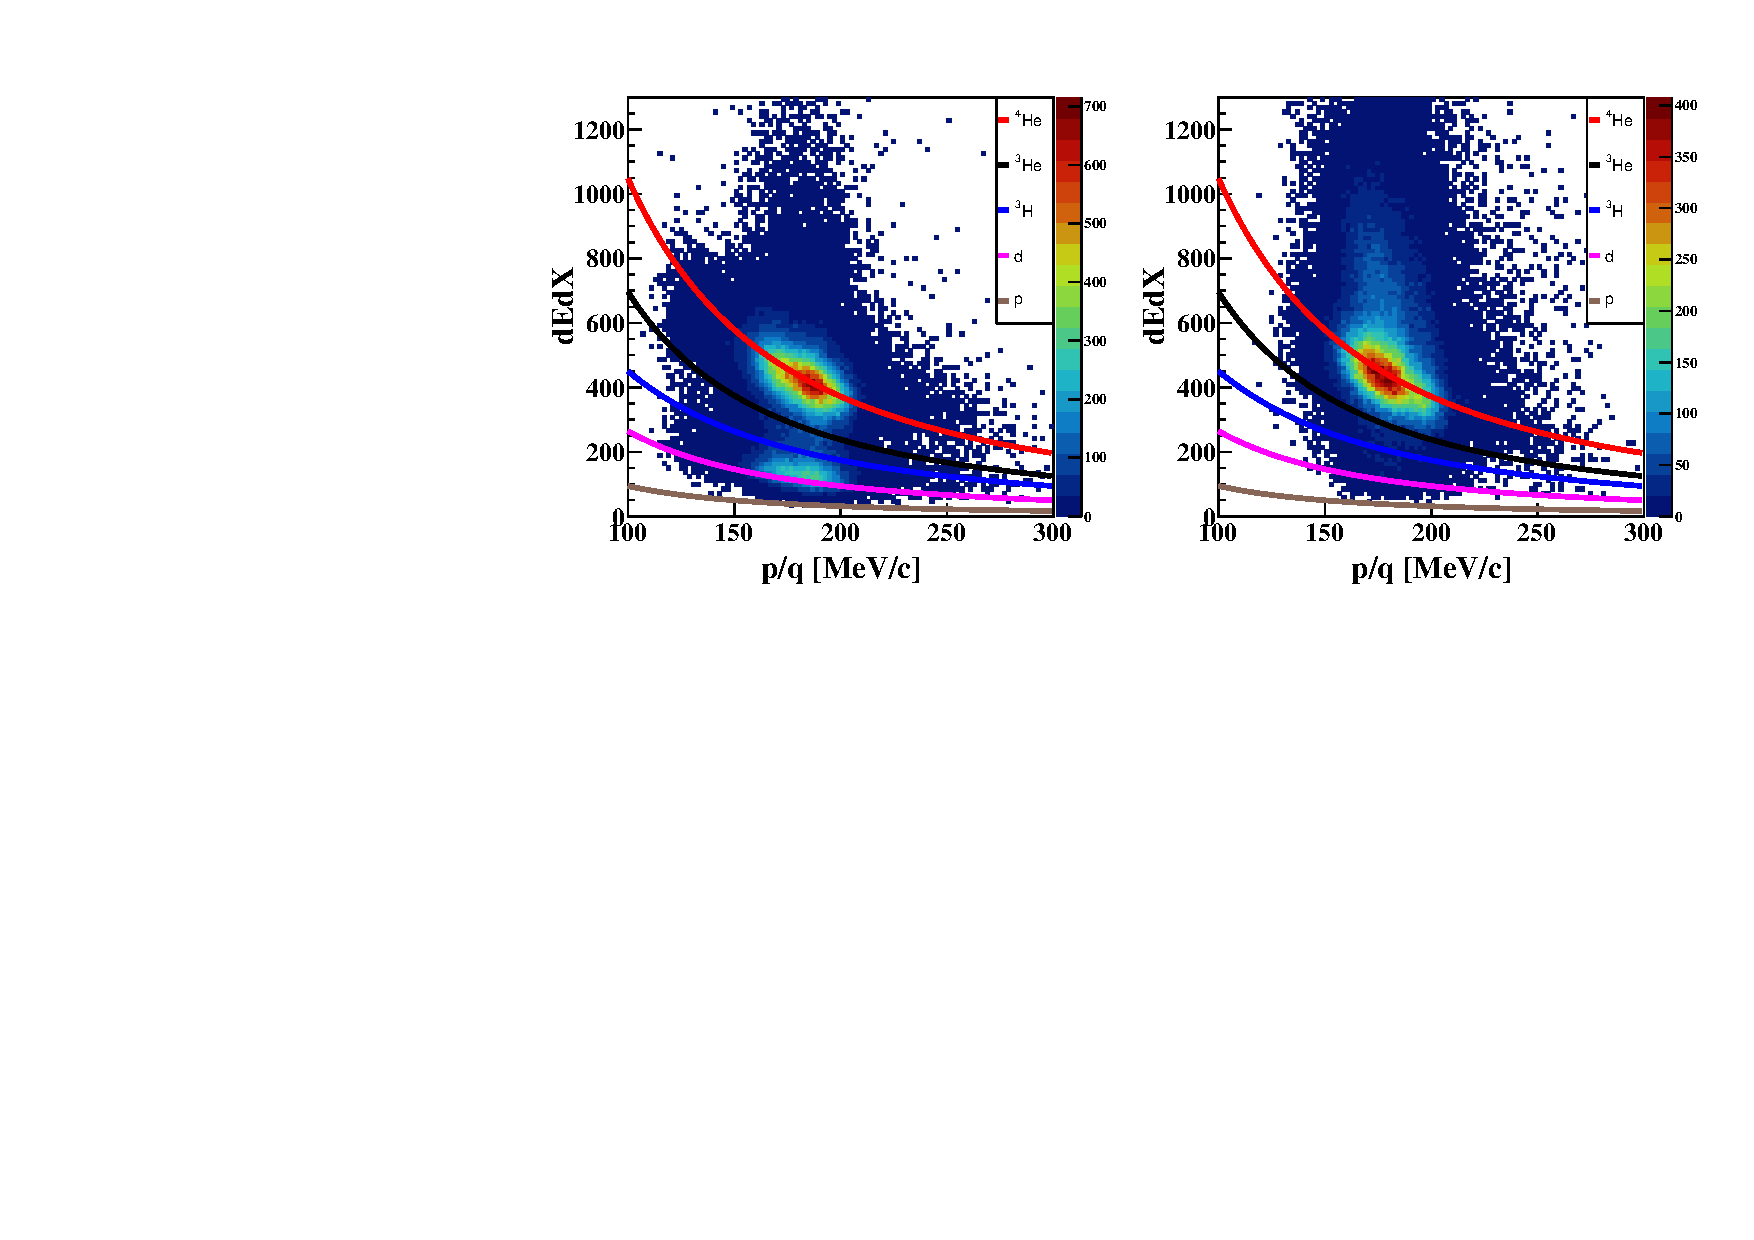
\includegraphics[scale=0.73]{f_dedx_p_exp_2nd.pdf}
\caption{$\small{\frac{dE}{dX}}$ vs. $p/q$ distributions for the left (on the 
   left) and for the right (on the right) half of the RTPC after gain 
   calibration. The lines are theoretical expectations from the Bethe-Bloch 
   formula for $^4$He 
   (red), $^3$He (black), $^3$H (blue), $^2$H (pink) and protons (gray).}
\label{fig:dedx_p_exp_2nd}
\end{figure*}

\section{Track Reconstruction}
\label{sec_tracking}

\subsection{Noise Rejection}
Two independent noise signatures were identified in the raw data and removed 
in software prior to track reconstruction. Both are transient and isolated to 
a subset of the readout channels. 

The first is an oscillatory noise located early in the readout time window, 
shown in the top panel of Figure~\ref{fig:noise} for a particularly noisy 
channel. Its amplitude is similar to those of real tracks. About 18\% of the 
readout channels exhibit large contributions from this noise.  
Due to its unique time-energy correlation, we use a patern
recognition algorithm and discard the hits coming from the channels that display 
this behavior on an event by event basis. The result of the
procedure is illustrated in the bottom panel of Figure~\ref{fig:noise}.

The second noise signature was a coherent noise affecting about 25\% of the 
pre-amplifiers boards, when simultaneous hits in most of the 16 channels of the
board were recorded. An event-based technique to identify and remove this noise 
was developed based 
on counting simultaneous hits in each pre-amplifier group, and, if sufficiently large, 
perform a dynamic pedestal subtraction based on the average ADC of neighboring 
channels within this group.

The sources of these effects were not determined, but rejection techniques 
allowed to reconstruct 10\% more good tracks and 
recover 70 channels that were previously ignored due to excessive noise levels.

\begin{figure}[tb]
   \centering
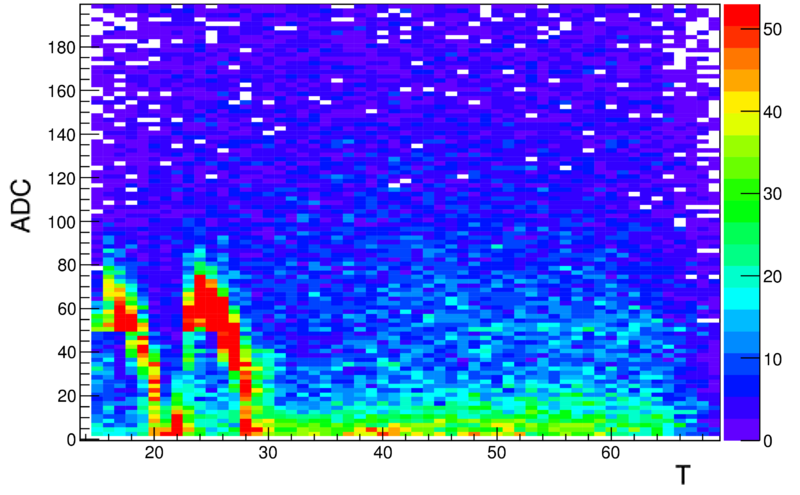
\includegraphics[scale=0.25]{noisy_pad_before_rejection2.png}
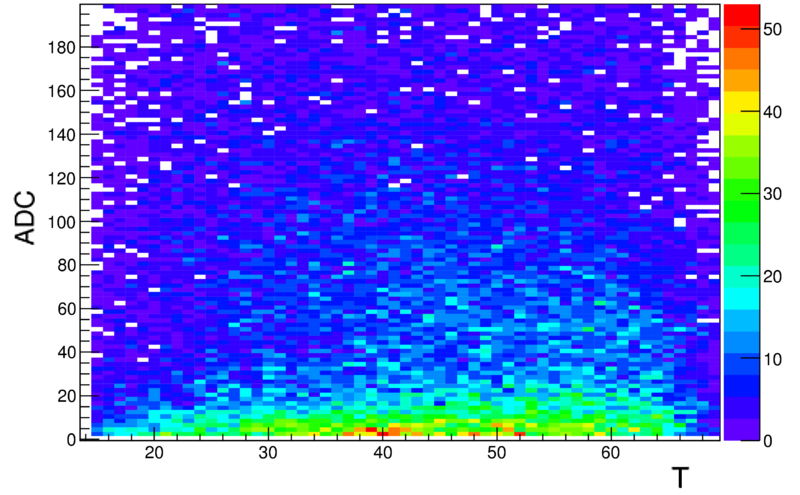
\includegraphics[scale=0.25]{noisy_pad_after_rejection2.png}
\caption{The ADC vs. T spectrum for an example noisy channel before (top) and 
after (bottom) noise rejection algorithms.  Only hits associated with tracks 
are included, and the selection of events and tracks is the same in both 
plots.}
\label{fig:noise}
\end{figure}


\subsection{Track Fitting}\label{sec_rec}

The tracking starts with reconstructing the spacial origin of the hits using the extracted drift speed and drift path 
parameters. For each registered hit, we calculate a position of emission from 
the signal time and the pad position. The third step 
is to create chains of hits. The maximum distance between two close adjacent 
hits has to be less than 10.5 mm to chain them, which roughly corresponds to 
neighbors and next to neighbors. We fit the chains with a helix if they have a minimum of 
10 hits. We then eliminate from the chain the hits that are 5 mm or farther from the fit,
as they are not likely part of the same track.
This new reduced chain is used for a second and final helix fit.

For energy deposition, the mean $\frac{dE}{dx}$ is calculated as
\begin{equation}
 \left\langle \frac{dE}{dX} \right\rangle= \frac{\sum\limits_{i} \frac{ADC_{i}}{G_i}}{L},
\end{equation}
where the sum runs over all the hits of the track, $G_{i}$ is the gain of 
the associated pad, and $L$ is the visible track length in the active drift 
volume. 

\subsection{Energy Loss Corrections}\label{sec_eloss}
Energy loss between the target and drift region was significant in the RTPC and 
necessitated a correction for optimal momentum reconstruction at the primary 
interaction vertex.  The dominant loss was in the 27~\textmu{}m thick Kapton target 
wall, with significant contributions also from the pressurized target gas and 
the foils before reaching the drift region.  Corrections were developed based 
on GEANT4 simulations with the full RTPC geometry and parameterized in terms of 
recoil curvature in the drift region and polar angle, separetely for all recoil 
hypotheses ($p$, $d$, $^3$H, $^3$He, $^4$He).  At our average coherent $^4$He 
DVCS kinematics, energy losses were about 5 MeV, while for $e-^4$He elastic 
scattering losses were about 3 MeV, which corresponds to momentum corrections 
of 25\% and 15\%, respectively.

\section{Performance Studies}\label{sec_perfor}

The primary data sample used for calibration and performance assessment of the
RTPC was elastic scattering with a 1.2 GeV electron beam. The electron momentum
and direction is measured with CLAS, which uniquely determines the expected recoiling
$^4$He kinematics. Matching requirements between reconstructed and expected $z$-vertex
and direction of the RTPC track provides a clean selection of elastically-scattered
$^4$He, shown in Figure~\ref{fig:w}.

\begin{figure}[tb]\centering
  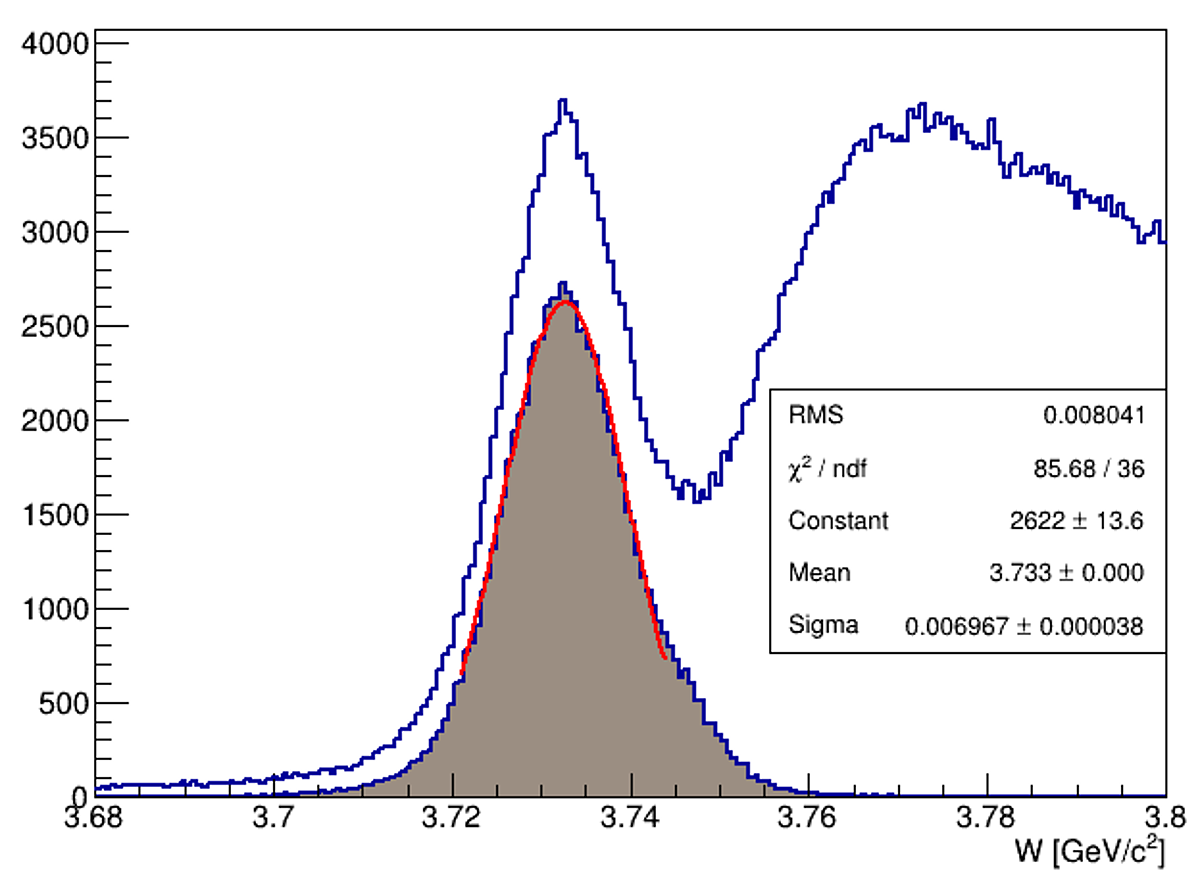
\includegraphics[width=8cm]{fit_W_distribution_l.png}
  \caption{The recoil mass $W$ distribution calculated from electron kinematics 
  before (``inclusive'') and after (``exclusive'') requiring a matching track 
  in the RTPC.\label{fig:w}}
\end{figure}


\subsection{Resolution}

Elastic scattering was used to estimate the tracking resolution of the RTPC 
based on the residual between the expected and measured $^4$He tracks.  The RTPC
resolutions, after removing contributions from the electron, are shown in Table
~\ref{tab:reso}, and are very similar for the two halves of the RTPC.  Note that the
$\theta$- and $z$-resolutions are highly correlated.

\begin{table}[htbp]
\begin{center}
\begin{tabular}{|l|cccc|}
  \hline
& $\sigma_{z}$ &  $\sigma_{\theta}$ & $\sigma_{\phi}$ & $\sigma_{p}/p$\\
\hline
Left &  5.3 mm & 3.8$^{\circ}$ & 1.9$^{\circ}$ & 9$\%$ \\
Right & 6.5 mm & 4.0$^{\circ}$ & 1.9$^{\circ}$ & 8$\%$\\
\hline
\end{tabular}
\caption{The resolutions of the two modules of the RTPC for $z$-vertex, 
polar and azimuthal angles, and momentum.}
\label{tab:reso}
\end{center}
\end{table}


\subsection{Efficiency}

We measured the efficiency of the RTPC
using elastic scattering on $^4$He by comparing the inclusive yield, based
only on electron detection, to the exclusive elastic yield, where the Helium
recoil is also detected (see Figure~\ref{fig:w}). We present in 
Figure~\ref{fig:rtpc_eff} the results for the two halves of the detector. We 
observe that the left and the right modules have similar efficiencies except 
near the upstream target window. This difference is due to the large number of 
dead channels concentrated in this part of the left half of the detector

\begin{figure}[tb]
\centering
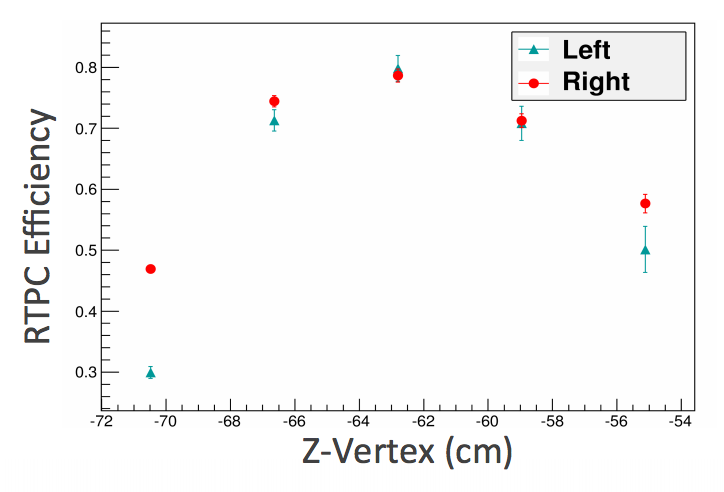
\includegraphics[width=8cm]{tpceff.png}
\caption{The RTPC $^4$He detection efficiency as a function of the longitudinal 
   position along the detector.
 \label{fig:rtpc_eff}}
 \end{figure}


 \section{Conclusion}

We reported on the construction, operation and calibration of a small RTPC 
designed to measure $^4$He nuclei in high rate environment. The operation
of the detector was successful and allowed to detect Helium nuclei with a 75\%
efficiency and a readout rate
of 3.1 kHz triggered by the detection of high energy electrons and 
photons in the CLAS spectrometer. 

\input acknowledgment.tex  

\begin{thebibliography}{99}

\bibitem{Mecking:2003zu} 
   B.~A.~Mecking {\it et al.} [CLAS Collaboration],
  The CEBAF Large Acceptance Spectrometer (CLAS),
  Nucl.\ Instrum.\ Meth.\ A {\bf 503}, 513 (2003).
  %doi:10.1016/S0168-9002(03)01001-5

\bibitem{Mestayer:2000we} 
   M.~D.~Mestayer {\it et al.},
  The CLAS drift chamber system,
  Nucl.\ Instrum.\ Meth.\ A {\bf 449}, 81 (2000).
  %doi:10.1016/S0168-9002(00)00151-0

\bibitem{Adams:2001kk} 
   G.~Adams {\it et al.},
  The CLAS Cherenkov detector,
  Nucl.\ Instrum.\ Meth.\ A {\bf 465}, 414 (2001).
  %doi:10.1016/S0168-9002(00)01313-9

\bibitem{Smith:1999ii} 
   E.~S.~Smith {\it et al.},
  The time-of-flight system for CLAS,
  Nucl.\ Instrum.\ Meth.\ A {\bf 432}, 265 (1999).
  %doi:10.1016/S0168-9002(99)00484-2

\bibitem{Amarian:2001zs} 
   M.~Amarian {\it et al.},
  The CLAS forward electromagnetic calorimeter,
  Nucl.\ Instrum.\ Meth.\ A {\bf 460}, 239 (2001).
  %doi:10.1016/S0168-9002(00)00996-7

\bibitem{Girod:2007aa} 
   F.~X.~Girod {\it et al.} [CLAS Collaboration],
  Measurement of Deeply virtual Compton scattering beam-spin asymmetries,
  Phys.\ Rev.\ Lett.\  {\bf 100}, 162002 (2008).
  %doi:10.1103/PhysRevLett.100.162002
  %[arXiv:0711.4805 [hep-ex]].

\bibitem{Hyon-suk}
   Hyon-Suk Jo, Etude de la Diffusion Compton Profond{\'e}ment Virtuelle Sur le 
   Nucl{\'e}on avec le D{\'e}tecteur CLAS de Jefferson Lab: Mesure des Sections 
   Efficaces polaris{\'e}es et non polaris{\'e}es, IPNO-Thesis (2007).

\bibitem{proposal1}
   G.~Asryan et al., Meson spectroscopy in the Coherent Production on $^{4}$He 
   with CLAS, Jlab proposal to PAC31 (2007).

\bibitem{proposal2}
   K.~Hafidi et al., Deeply virtual Comton scattering off $^{4}$He, Jlab 
   proposal to PAC33 (2008).

\bibitem{Fenker:2008zz} 
   H.~C.~Fenker {\it et al.},
  BoNuS: Development and Use of a Radial TPC using Cylindrical GEMs,
  Nucl.\ Instrum.\ Meth.\ A {\bf 592}, 273 (2008).
  %doi:10.1016/j.nima.2008.04.047

\bibitem{Sauli:2016eeu} 
   F.~Sauli,
  The gas electron multiplier (GEM): Operating principles and applications,
  Nucl.\ Instrum.\ Meth.\ A {\bf 805}, 2 (2016).
  %doi:10.1016/j.nima.2015.07.060

\bibitem{Bachmann:2000kj} S.~Bachmann {\it et al.},
 Performance of GEM detectors in high intensity particle beams,
 Nucl.\ Instrum.\ Meth.\ A {\bf 470}, 548 (2001).
 %doi:10.1016/S0168-9002(01)00802-6

\bibitem{Biagi:1999nwa} 
   S.~F.~Biagi,
  Monte Carlo simulation of electron drift and diffusion in counting gases 
  under the influence of electric and magnetic fields,
  Nucl.\ Instrum.\ Meth.\ A {\bf 421}, no. 1-2, 234 (1999).
  %doi:10.1016/S0168-9002(98)01233-9

 \bibitem{ALICE-FEE}
 L. Musa et al., The ALICE TPC front end Electronics, Nuclear Science Symposium 
 Conference Record, 2003 IEEE, 5 3647-3651 Vol.5, Oct (2003).
 
%\bibitem{Soltveit:2012jp} 
%   H.~K.~Soltveit {\it et al.},
%  The Preamplifier shaper for the ALICE TPC-Detector,
%  Nucl.\ Instrum.\ Meth.\ A {\bf 676}, 106 (2012).
  %doi:10.1016/j.nima.2012.02.012
  %[arXiv:1203.3564 [physics.ins-det]].
 
\bibitem{EsteveBosch:2003bj} 
   R.~Esteve Bosch, A.~Jimenez de Parga, B.~Mota and L.~Musa,
  The ALTRO chip: A 16-channel A/D converter and digital processor for gas 
  detectors,
  IEEE Trans.\ Nucl.\ Sci.\  {\bf 50}, 2460 (2003).
  %doi:10.1109/TNS.2003.820629
\bibitem{RCU}
    C.~G.~Gutierrez et al., The ALICE TPC Readout Control Unit, IEEE Nuclear Science Symposium Conference Record, 1, 575 



\bibitem{GEANT4}
http://geant4.cern.ch
 	

\end{thebibliography}

\end{document}

